\section{Konfiguracja projektu}
\label{sec:vivado-conf}
http://svenand.blogdrive.com/archive/169.html

https://embeddedgreg.com/2014/03/13/step-1-hardware-design-for-zybo/

\subsection{Podstawowa konfiguracja projektu}

Wykorzystany w projekcie układ - Digilent ZYBO - nie jest bezpośrednio wspierany przez środowisko Vivado. Wynika z tego konieczność sprecyzowania parametrów układu na etapie tworzenia projektu. W trakcie modyfikowania projektu, w przypadku dodania modułów wykorzystujących interfejs wejścia/wyjścia, konieczna jest również konfiguracja parametrów interfejsu. Aby uprościć proces projektowania, zalecane jest skonfigurowanie obsługi układu przed utworzeniem projektu. Proces ten opisano w dokumentacji producenta. \cite{zybo-in-vivado}

\subsubsection{Vivado}

Utworzyć należy projektu typu \emph{,,RTL Project''}, z odznaczoną opcją \emph{,,Do not specify sources at this time''}.

W kroku \emph{,,Add Constraints''} dodać należy plik konfiguracyjny dla wybranego układu. W przypadku ZYBO, plik ten jest dostępny na stronie producenta. W kolejnym kroku możliwe jest skonfigurowanie parametrów układu. Wykorzystać do tego należy zakładkę \emph{,,Boards''} i wybrać wykorzystywany model.

Po utworzeniu projektu, skonfigurować należy właściwą przestrzeń roboczą dla projektu, wykorzystując do tego opcję \emph{,,IP Integrator -> Create Block Design''}.

Do nowo utworzonej przestrzeni dodać należy moduł IP reprezentujący procesor ZYNQ - \emph{,,ZYNQ7 Processing System''}.

W kolejnych krokach należy dokonać konfiguracji modułu procesora, klikając dwukrotnie na moduł.

\begin{itemize}
	\item Kanały interfejsu AXI mogą być konfigurowane przez zakładkę \emph{,,PS-PL Configuration''}. Możliwa jest aktywacja kanałów ogólnego przeznaczenia (\emph{GP}), oraz wysokiej wydajności (\emph{HP}).
	
	\item Interfejsy komunikacji konfigurowane mogą być z poziomu zakładki \emph{,,MIO Configuration''}. Zalecane jest aktywowanie interfejsów \emph{ENET 0}, \emph{SD 0} i \emph{UART 1} ze względu na ich wykorzystanie na dalszym etapie pracy.
	
	Przykład konfiguracji interfejsów wejścia/wyjścia przedstawiono na rysunku \ref{fig:vivado-mio-configuration}.
	\begin{figure}[ht]
		\centering
		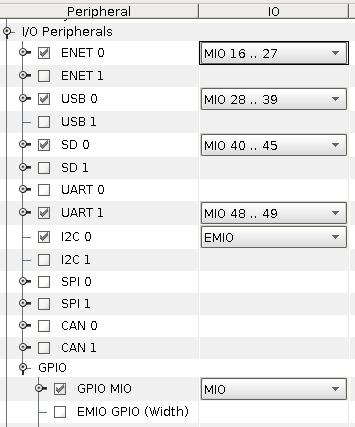
\includegraphics[height=8cm]{img/vivado/mio-configuration.png}
		\caption{Okno konfiguracji interfejsów wejścia i wyjścia.}
		\label{fig:vivado-mio-configuration}
	\end{figure}
	
	\item Parametry sygnałów zegarowych dostępnych z poziomu układów logiki reprogramowalnej modyfikować można w zakładce \emph{,,Clock Configuration/PL Fabric Clocks''}.
	
	\item Częstotliwość pracy procesora oraz pamięci zmienić można w zakładce \emph{,,Clock Configuration/Processor/Memory Clocks''}.
\end{itemize}

Po ukończeniu etapu konfiguracji procesora i powrocie do głównego okna programu, należy użyć opcji \emph{,,Run Block Automation''}. Utworzone zostaną połączenia interfejsów pamięci \texttt{DDR} oraz \texttt{FIXED\_IO}.

W przypadku zdefiniowania interfejsów AXI, połączyć należy właściwe sygnały zegarowe. Przykład wynikowej konfiguracji projektu przedstawiono na rysunku \ref{fig:vivado-config-result}.

	\begin{figure}[ht]
		\centering
		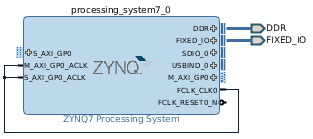
\includegraphics[]{img/vivado/vivado-config-result.png}
		\caption{Okno projektu.}
		\label{fig:vivado-config-result}
	\end{figure}
	
Przedstawiona konfiguracja stanowi podstawę każdego projektu wykorzystującego moduł procesora ZYNQ.

Po zakończeniu konfiguracji, wygenerować należy warstwę HDL, korzystając z opcji \emph{,,Create HDL Wrapper''} dostępnej po kliknięciu prawym przyciskiem myszy na utworzony wcześniej plik źródłowy.

Skonfigurowany w ten sposób projekt może być budowany i uruchamiany na platformie ZYBO.
\subsubsection{SDK}

W celu utworzenia projektu aplikacji w SDK, konieczne jest wyeksportowanie plików opisujących projekt z poziomu Vivado, wykorzystując do tego opcję \emph{,,File/Export/Export Hardware''} z zaznaczoną opcją \emph{,,Include bitstream''}.

W efekcie, dostępna powinna być aplikacja \texttt{\textit{nazwa\_projektu}\_hw\_platform\_0}, zawierająca plik \texttt{nazwa\_projektu.hdf}. Aplikacja ta stanowi podstawę każdego budowanego programu bare-metal.

W przypadku budowania aplikacji na platformę PetaLinux, na etapie tworzenia projektu, zmodyfikować należy pole \emph{,,OS Platform''} na wartość \emph{,,linux''}, \emph{,,Processor Type''} na \emph{,,ps7\_cortexa9''}, oraz wybrać właściwy język programowania.

W kontekście tak utworzonej aplikacji nie znajdują się biblioteki dostarczane przez firmę \emph{Xilinx}, wykorzystywane w aplikacjach bare metal, dostępna jest jednak pełna biblioteka języka \emph{C} oraz \emph{C++}.

W celu uruchomienia aplikacji systemowej na platformie ZYBO, przeprowadzić należy proces budowania i skopiować wynikowy plik z katalogu \texttt{Debug} lub \texttt{Release} do systemu plików systemu PetaLinux. Wykorzystać można do tego narzędzie SSH:

\begin{lstlisting}[breaklines=true]
scp Debug/hello-world.elf root@adres-ip:~/
\end{lstlisting}

Aplikację uruchomić można przy użyciu konsoli użytkownika, również stosując narzędzie SSH.
\subsubsection{PetaLinux}
\label{sec:petalinux-config}

Utworzenie struktury katalogów projektu wykonywane jest przy użyciu poniższego polecenia.

\begin{lstlisting}[breaklines=true]
petalinux-create -t project --template zynq --name (*@\textit{nazwa-projektu}@*)
cd (*@\textit{nazwa-projektu}@*)
\end{lstlisting}

Powstała struktura zintegrowana jest z systemem kontroli wersji \emph{git}, co pozwala utrzymać uporządkowanie danych wewnątrz projektu oraz wersjonowanie. Zarządzanie repozytorium wykorzystuje podstawowe komendy narzędzia.

Kolejnym krokiem jest zaimportowanie projektu \emph{Vivado}.

\begin{lstlisting}[breaklines=true]
petalinux-config --get-hw-description=(*@\textit{/sciezka/do/projektu/projekt.sdk/}@*)
\end{lstlisting}

Jeśli polecenie wywołane zostało po raz pierwszy dla danego projektu, uruchomione zostanie narzędzie konfiguracyjne, domyślne ustawienia są jednak poprawne.

Konfiguracja projektu odbywa się przy użyciu polecenia \texttt{petalinux-config}.
Skonfigurować należy metodę uruchamiania systemu - w omawianym przypadku, uruchomienie następuje na bazie plików znajdujących się na karcie SD.
\begin{lstlisting}[breaklines=true]
petalinux-config
Image Packaging Configuration ---> Root filesystem type ---> SD card
\end{lstlisting}

Następnie, przeprowadzić należy proces budowania systemu oraz wygenerować pliki wynikowe.

\begin{lstlisting}[breaklines=true]
petalinux-build
petalinux-package --boot --fsbl images/linux/zynq_fsbl.elf --fpga images/linux/system_wrapper.bit --u-boot --force
petalinux-package --image -c rootfs --format initramfs
\end{lstlisting}

Uruchomienie systemu wymaga przygotowania karty SD - musi ona posiadać dwie partycje, pierwszą, z etykietą \emph{boot} i systemem plików \emph{fat32}, drugą - odpowiednio \emph{sys} i \emph{ext4}. Pierwsza z nich, zawierająca pliki wymagane na etapie inicjalizacji systemu, musi być poprzedzona 4 MB niezaalokowanej przestrzeni i mieć rozmiar co najmniej 40 MB. Druga partycja zawiera pliki systemowe, jej rozmiar powinien wynosić co najmniej kilkaset megabajtów. Proces formatowania przeprowadzić można przy użyciu narzędzia \emph{gparted}.

Pliki wynikowe należy przenieść na kartę SD, korzystając z poleceń.

\begin{lstlisting}[breaklines=true]
rm -rf /(*@\textit{punkt-montowania}@*)/sys/*
cp images/linux/BOOT.BIN /(*@\textit{punkt-montowania}@*)/boot/
cp images/linux/image.ub /(*@\textit{punkt-montowania}@*)/boot/
cp images/linux/rootfs.cpio /(*@\textit{punkt-montowania}@*)/sys/
cd /(*@\textit{punkt-montowania}@*)/
pax -rvf rootfs.cpio
sync
cd -
\end{lstlisting}

Ze względu na mechanizm buforowania przez kontroler operacji zapisu danych, pamiętać należy o wywołaniu polecenia \texttt{sync}, zapewniającego zachowanie integralności danych.

Karta SD pozwala na uruchomienie systemu operacyjnego na układzie i przechowywanie danych użytkownika pomiędzy startami układu. Dalsza praca z systemem odbywać się może przez protokoły komunikacji \emph{SSH} lub \emph{UART}.

\subsection{Konfiguracja modułu AXI DMA}
\label{sec:vivado-axi-dma}

\subsubsection{Vivado}
Oprogramowanie Vivado umożliwia zbudowanie modułu wykorzystującego protokół AXI przez użycie opcji \emph{Create and package new IP...}, zawartej w menu \emph{Tools}.

Na ekranie wyboru zadania wybrać należy opcję \emph{Create a new AXI4 peripheral}.

Po zdefiniowaniu podstawowych danych związanych z modułem, takich jak jego nazwa i nazwisko autora, w kolejnym kroku możliwe będzie zdefiniowanie interfejsu modułu. Na tym etapie konfiguracji skonfigurować należy wszystkie połączenia wykorzystujące interfejs AXI.

W przypadku modułu konfiguracyjnego o podstawowej strukturze, interfejs zawierać powinien jedno połączenie wykorzystujące protokół AXI w wersji \emph{Lite}, działający w trybie \emph{slave}, z oczekiwaną liczbą rejestrów. Każdy rejestr powinien być związany z jedną wartością, której konfiguracja ma być możliwa. Przykład konfiguracji przedstawiono na rysunku \ref{fig:axi-dma-interfaces-conf}.

\begin{figure}[h]
	\centering
	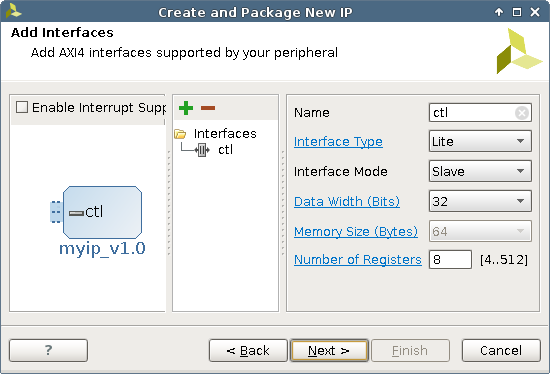
\includegraphics[width=8cm]{img/vivado/axi-dma-interfaces-conf.png}
	\caption{Konfiguracja interfejsów modułu AXI DMA.}
	\label{fig:axi-dma-interfaces-conf}
\end{figure}

W omawianym przykładzie zdefiniowano interfejs AXI o nazwie \emph{ctl}, związany z ośmioma rejestrami o długości trzydziestu dwóch bitów w pamięci.

Zdefiniowanie interfejsów kończy proces podstawowej konfiguracji modułu. W kolejnym kroku należy wybrać opcję \emph{Edit IP} w celu dostosowania kodu źródłowego modułu.

Po wygenerowaniu, z modułem powinien być związany jeden plik źródłowy, zwierający instrukcje odpowiadające za obsługę komunikacji przy użyciu interfejsu AXI.

Do pliku dodać należy elementy odpowiedzialne za zdefiniowanie wyjść modułu oraz przypisanie im właściwych wartości.

W celu zdefiniowania wyjść modułu, odpowiadające im wpisy należy umieścić po komentarzu \emph{,,// Users to add ports here''}. Przykład przedstawiono na listingu \ref{listing:axi-dma-outputs}.

\begin{lstlisting}[breaklines, label=listing:axi-dma-outputs, caption=Definicja interfejsów wyjściowych modułu.]
// Users to add ports here
output wire parameter_a,
output wire [7:0] parameter_b,
output wire [15:0] parameter_c,
output wire [31:0] parameter_d,
// User ports ends
\end{lstlisting}

Zdefiniowano cztery sygnały wyjściowe, o różnej liczbie bitów.

Następnie, należy dokonać modyfikacji kodu odpowiedzialnej za powiązanie wartości parametrów z rejestrami modułu. Rejestry AXI zdefiniowane są poniżej linii \emph{,,//-- Number of Slave Registers N''}, gdzie \emph{N} to liczba dostępnych rejestrów. Rejestry te mają nazwy \texttt{slv\_reg\emph{n}}, gdzie \emph{n} to indeks rejestru, i nie jest zalecana modyfikacja tych nazw.

Modyfikacji kodu należy dokonać poniżej linii \emph{,,// Add user logic here''}. Przykład przedstawiono na listingu \ref{listing:axi-dma-associate}.

\begin{lstlisting}[breaklines, label=listing:axi-dma-associate, caption=Powiązanie wyjść z rejestrami modułu.]
// Add user logic here
assign parameter_a = slv_reg0[0];
assign parameter_b = slv_reg1[7:0];
assign parameter_c = slv_reg2[15:0];
assign parameter_d = slv_reg3[31:0];
// User logic ends
\end{lstlisting}

W przedstawionym przykładzie powiązano wartości parametrów bezpośrednio z danymi znajdującymi się w rejestrach. W rozbudowanych aplikacjach może być konieczne dodanie instrukcji modyfikujących wartości rejestrów przed przesłaniem ich na wyjście modułu.

Po ukończeniu modyfikacji modułu, konieczne jest zapisanie zmian i wygenerowanie plików wynikowych. W tym celu, należy wykorzystać okno \emph{Package IP}, sekcję \emph{Review and Package}. Widok okna przedstawiono na rysunku \ref{fig:axi-dma-review-package}.

\begin{figure}[ht]
	\centering
	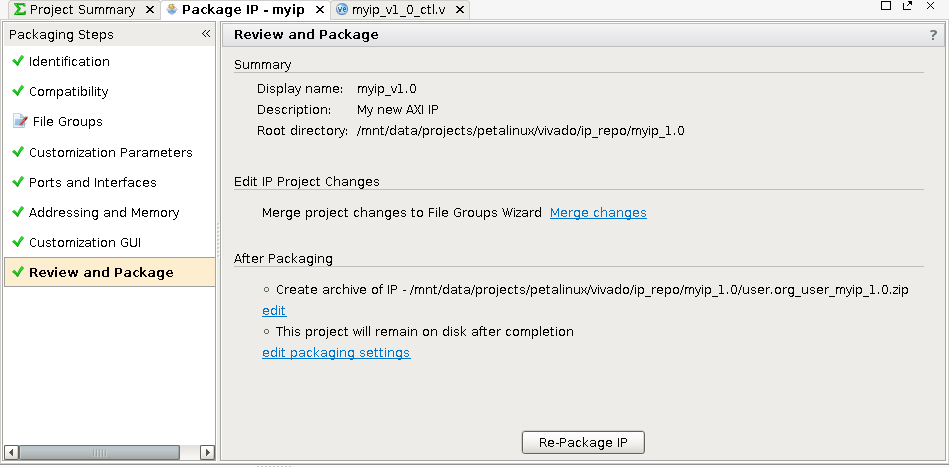
\includegraphics[width=12cm]{img/vivado/axi-dma-review-package.png}
	\caption{Okno finalizacji modyfikacji modułu.}
	\label{fig:axi-dma-review-package}
\end{figure}

Należy wybrać opcję \emph{Merge changes}, umożliwiającą zintegrowanie wprowadzonych zmian z projektem bazowym. Następnie, można zakończyć edycję projektu przez wybór opcji \emph{Re-Package IP}. Moduł będzie dostępny z poziomu interefejsu wyszukiwania modułów IP.

\subsubsection{SDK}
Konfiguracja wartości parametrów modułu opiera się na zapisie do właściwych sektorów pamięci. W przypadku pracy w trybie \emph{base metal}, wykorzystać można instrukcję \emph{Xil\_Out32} z biblioteki \emph{xil\_io.h}. W przypadku pracy z systemem \emph{PetaLinux}, wykorzystać należy biblioteki systemowe. Implementację \emph{bare metal} przedstawiono na listingu \ref{listing:axi-dma-bare-metal}, natomiast systemową na listingach \ref{listing:axi-dma-petalinux-main}, \ref{listing:axi-dma-petalinux-axi-h} i \ref{listing:axi-dma-petalinux-axi-c}.

\begin{lstlisting}[breaklines, language=C, label=listing:axi-dma-bare-metal, caption=Obsługa modułu w trybie \emph{bare metal}.]
#include "xparameters.h"
#include "platform.h"
#include "xil_io.h"

#define PARAMETER_A_REGISTER 0
#define PARAMETER_B_REGISTER 4
#define PARAMETER_C_REGISTER 8
#define PARAMETER_D_REGISTER 12

#define BASEADDR XPAR_ALGORITHM_PARAMETERS_0_CTL_BASEADDR

int main()
{
	init_platform();
	
	Xil_Out32(BASEADDR + PARAMETER_A_REGISTER, 1);
	Xil_Out32(BASEADDR + PARAMETER_B_REGISTER, 25);
	Xil_Out32(BASEADDR + PARAMETER_C_REGISTER, 1 << 10);
	Xil_Out32(BASEADDR + PARAMETER_D_REGISTER, 1 << 30);
	
	while(1);
}
\end{lstlisting}


\begin{lstlisting}[breaklines, language=C, label=listing:axi-dma-petalinux-main, caption=Obsługa modułu w trybie systemowym - \texttt{main.c}.]
#include <fcntl.h>
#include <stdio.h>
#include <stdlib.h>
#include <sys/mman.h>

#include "axi.h"

#define PARAMETER_A_REGISTER 0
#define PARAMETER_B_REGISTER 4
#define PARAMETER_C_REGISTER 8
#define PARAMETER_D_REGISTER 12

#define BASEADDR 0x43000000

typedef int memory_handle_t;

void setup_virtual_memory(struct axi_interface *interface, size_t length, memory_handle_t memory_handle, off_t base_addr) {
	interface->base_addr = base_addr;
	interface->virt_addr = (virt_address) mmap(NULL, length, PROT_READ | PROT_WRITE, MAP_SHARED, memory_handle, base_addr);
	if (interface->virt_addr == MAP_FAILED) {
		perror("Failed to map virtual memory.");
		exit(1);
	}
}

int main() {
	memory_handle_t memory_handle = open("/dev/mem", O_RDWR | O_SYNC);
	
	struct axi_interface* parameters = (struct axi_interface*) malloc(sizeof(struct axi_interface));
	if (parameters == NULL) {
		perror("Memory allocation failed.");
		exit(1);
	}
	setup_virtual_memory(parameters, 65535, memory_handle, BASEADDR);
	
	axi_write(parameters->virt_addr, PARAMETER_A_REGISTER, 1);
	axi_write(parameters->virt_addr, PARAMETER_B_REGISTER, 25);
	axi_write(parameters->virt_addr, PARAMETER_C_REGISTER, 1 << 10);
	axi_write(parameters->virt_addr, PARAMETER_D_REGISTER, 1 << 30);
	
	while(1);
}
\end{lstlisting}

\begin{lstlisting}[breaklines, language=C, label=listing:axi-dma-petalinux-axi-h, caption=Obsługa modułu w trybie systemowym - \texttt{axi.h}.]
#include <stdbool.h>

typedef unsigned int* virt_address;

struct axi_interface {
	unsigned int base_addr;
	virt_address virt_addr;
};

void axi_write(virt_address virt_addr, int location, unsigned int value);
\end{lstlisting}

\begin{lstlisting}[breaklines, language=C, label=listing:axi-dma-petalinux-axi-c, caption=Obsługa modułu w trybie systemowym - \texttt{axi.c}.]
#include "axi.h"

void axi_write(virt_address virt_addr, int location, unsigned int value) {
	virt_addr[location >> 2] = value;
}
\end{lstlisting}

\subsubsection{PetaLinux}
W celu wykorzystania techniki DMA w aplikacji działającej w systemie PetaLinux, konieczna jest aktywacja właściwych parametrów konfiguracji na etapie budowania systemu. W tym celu wykonać należy polecenie:

\begin{lstlisting}[breaklines]
petalinux-config -c kernel
\end{lstlisting}

i aktywować funkcjonalność DMA:

\begin{lstlisting}[breaklines]
Device Drivers -> DMA Engine Support
Device Drivers -> DMA Engine Support -> Xilinx AXI DMAS Engine
\end{lstlisting}

\subsection{Obliczenia równoległe}
\label{sec:multithreading-config}
Użycie rozwiązań omawianych w rozdziale \ref{sec:openmp} wymaga aktywacji właściwych funkcji kompilacji.

W przypadku zastosowania wątków natywnych lub biblioteki dostępnej w standardzie C++ wymagane jest zastosowanie przełączników:

\begin{lstlisting}[language=bash]
g++ main.cpp -o main.out (*@\textbf{-pthread -std=c++11}@*)
\end{lstlisting}

Dla biblioteki TBB wymagane jest przeprowadzenie linkowania względem jej kodu źródłowego:

\begin{lstlisting}[language=bash]
g++ main.cpp -o main.out (*@\textbf{-ltbb}@*)
\end{lstlisting}

Natomiast dla interfejsu OpenMP, konieczne jest użycie przełącznika:

\begin{lstlisting}[language=bash]
g++ main.cpp -o main.out (*@\textbf{-fopenmp}@*)
\end{lstlisting}
